\documentclass[11pt, oneside]{article} 
\usepackage{geometry}
\geometry{letterpaper} 
\usepackage{graphicx}
	
\usepackage{amssymb}
\usepackage{amsmath}
\usepackage{parskip}
\usepackage{color}
\usepackage{hyperref}

\graphicspath{{/Users/telliott_admin/Tex/png/}}
% \begin{center} 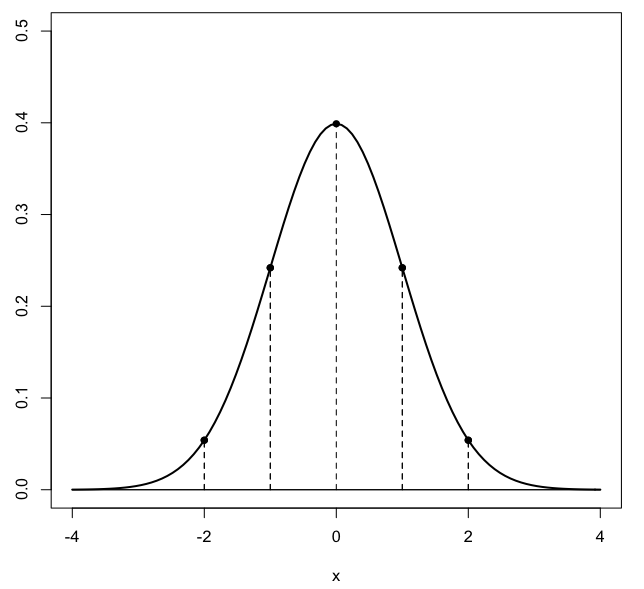
\includegraphics [scale=0.4] {gauss3.png} \end{center}

\title{Integer sums}
\date{}

\begin{document}
\maketitle
\Large

This chapter continues with a full treatment of formulas for sums of squares, cubes, and so on.  It is somewhat detailed, and can easily be skipped without loss of continuity.

\subsection*{Sum of Squares}
\begin{center} 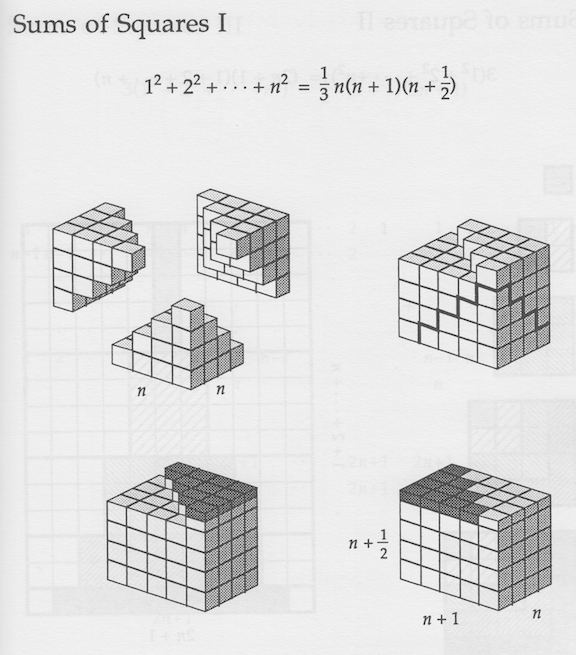
\includegraphics [scale=0.35] {sum_n2.png}\end{center}
We want the sum of the squares of the first $n$ integers.  There is a visual proof for this one as well (above).
\[ \sum_{k=1}^n k^2 \]
We obtain (by methods we will see below) the formula
\[ \sum_{k=1}^n k^2 = \frac{n(n+1)}{2} \frac{2n+1}{3} \]
\[ = \frac{n(n+1)(2n+1)}{6} \]
This formula is also written as
\[  \sum_{k=1}^n k^2 = \frac{1}{6} \ (2n^3 + 3n^2 + 2n) \]
\[ = \frac{n^3}{3} + \frac{n^2}{2} + \frac{n}{3} \]
We can check it by induction.  The base case is easy
\[ \frac{1(2)(3)}{6} = 1 \]  
$\checkmark$  

Now for the induction step:
\[ \frac{n(n+1)(2n+1)}{6} + (n+1)^2 \]
\[ = \frac{n+1}{6}  \ [ \ (n)(2n+1) + 6(n+1) \ ] \]
Look at what's in the brackets
\[ (n)(2n+1) + 6(n+1) \]
\[ = 2n^2 + 7n + 6 \]
\[ = (n + 2)(2n + 3) \]
\[ = (n + 1 + 1)(2(n + 1) + 1) \]
So altogether we have
\[ = \frac{(n+1)(n + 1 + 1)(2(n + 1) + 1)}{6} \]
which indeed, is the formula we had above, substituting $n+1$ for $n$.

\subsection*{Strang's proof}
Here are two more approaches.  The first one is in Strang's \emph{Calculus}.  He says "the best place to start is a good guess".  So again, our goal is to find a formula for:

\[ S = \sum_{k=1}^{n} \ k^2 \]

Perhaps we visualize a pile of cannonballs

\begin{center} 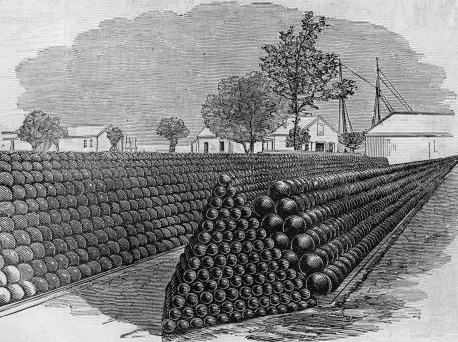
\includegraphics [scale=0.5] {cannonballs.png} \end{center}


Each layer contains a square number of cannonballs ($1$, then $4$, then $9$, etc.).  The shape is a pyramid with dimensions $n \times n \times n$.  We know the formula for the volume of a pyramid, and guess

\[ S_n = \frac{1}{3} n^3 \]

To test it, check whether this difference is $n^2$ (as it should be):

\[ S_{n} - S_{n-1} = \frac{1}{3} n^3 - \frac{1}{3} (n-1)^3 \]

Now

\[ (n-1)^2 = n^2 - 2n + 1 \]
\[ (n-1)^3 = (n-1)(n^2 - 2n + 1) \]
\[ = n^3 - 3 n^2 + 3 n - 1\]

So

\[ S_{n} - S_{n-1} = \frac{1}{3} (n^3 - n^3 + 3 n^2 - 3 n + 1) \]

We see that our guess is off by the residual terms

\[ \frac{1}{3} (3 n^2 - 3 n + 1) \]
\[ = n^2 - n + \frac{1}{3} \] 

Strang says:  the guess needs \emph{correction terms}.  
To cancel $1/3$ in the difference, subtract $n/3$ from the sum.  And to add back $n$ in the difference, add back $1 + 2 + \dots + n(n+1)/2$ to the sum.  Our new guess is

\[ S_n =  \frac{1}{3} n^3 + \frac{n(n+1)}{2} - \frac{n}{3} \]
\[ = \frac{n}{6} (2n^2 + 3(n+1) - 2) \]
\[ =  \frac{n}{6} (2n + 1)(n + 1) \]
\[ = \frac{n(n+1)(2n+1)}{6} \]

which may be easier to remember as

\[ S_n = \frac{n(n+1)}{2} \times \frac{2n + 1}{3} \]

\subsection*{Derivation by collapsing sum}

We proceed as we did in the case of the sum of integers.  There we used $(k+1)^2$ and worked out the consequences.  Here we use

\[ (k+1)^3 = k^3 + 3k^2 + 3k + 1 \]

We sum everything.

\[ \sum_{k=1}^n (k+1)^3 = \sum_{k=1}^n k^3 + \sum_{k=1}^n 3k^2 + \sum_{k=1}^n 3k + \sum_{k=1}^n 1 \]

As before, subtract the first term on the right from the left-hand side, giving us a collapsing sum.  We obtain

\[ \sum_{k=1}^n (k+1)^3 - \sum_{k=1}^n k^3 = (n+1)^3 - 1 \]
\[ = n^3 + 3n^2 + 3n \]

Recognize that the last sum is just $n$ 

\[ \sum_{k=1}^n 1 = n \]

subtract it from $3n$

\[ = n^3 + 3n^2 + 2n \]
\[ = n(n^2 + 3n + 2) \]
\[ = n(n+1)(n+2) \]

Assembling everything

\[ n(n+1)(n+2) = \sum_{k=1}^n 3k^2 + \sum_{k=1}^n 3k \]

We pull out the factor of $3$ from the sums

\[ n(n+1)(n+2) = 3\sum_{k=1}^n k^2 + 3\sum_{k=1}^n k  \]

The first sum on the right is what we seek, the second one is what we obtained before

\[ n(n+1)(n+2) = 3\sum_{k=1}^n k^2 + \frac{3}{2}\ n(n+1) \]

Multiply by $2$

\[ 2n(n+1)(n+2) = 6\sum_{k=1}^n k^2 + 3n(n+1) \]

Rearrange

\[ 6\sum_{k=1}^n k^2 = 2n(n+1)(n+2) - 3n(n+1) \]

Factor out the $n(n+1)$

\[ 6\sum_{k=1}^n k^2 = n(n+1) \ [ \ 2(n + 2) - 3 \ ] \]
\[ 6\sum_{k=1}^n k^2 = n(n+1)(2n + 1) \]
\[ \sum_{k=1}^n k^2 = \frac{n(n+1)}{2} \ \frac{(2n + 1)}{3}  \]

\subsection*{Sum of Cubes}

Let's do one more.  It will help in working out the Riemann Sum for $n^3$.  We proceed exactly as before

\[ (k+1)^4 = k^4 + 4k^3 + 6k^2 + 4k + 1 \]

Sum each term from $k=1 \rightarrow k=n$

\[ \sum_{k=1}^n (k+1)^4 = \sum_{k=1}^n k^4 + \sum_{k=1}^n 4k^3 + \sum_{k=1}^n 6k^2 + \sum_{k=1}^n 4k + \sum_{k=1}^n 1 \]

Rearrange and compute the collapsing sum.

\[ \sum_{k=1}^n (k+1)^4 - \sum_{k=1}^n k^4 = \sum_{k=1}^n 4k^3 + \sum_{k=1}^n 6k^2 + \sum_{k=1}^n 4k + \sum_{k=1}^n 1 \]

\[ (n+1)^4 - 1 = \sum_{k=1}^n 4k^3 + \sum_{k=1}^n 6k^2 + \sum_{k=1}^n 4k + \sum_{k=1}^n 1 \]

Substitute for the right-hand sum

\[ (n+1)^4 - 1 = \sum_{k=1}^n 4k^3 + \sum_{k=1}^n 6k^2 + \sum_{k=1}^n 4k + n \]

Rearrange some more

\[ \sum_{k=1}^n 4k^3 = (n+1)^4 - 1 - \sum_{k=1}^n 6k^2 - \sum_{k=1}^n 4k - n \]

Expand the term $(n+1)^4$ and pick up the $-1 - n$:

\[ (n+1)^4 - 1 - n \]
\[ = n^4 + 4n^3 + 6n^2 + 4n + 1 - 1 - n \]
\[ =  n^4 + 4n^3 + 6n^2 + 3n  \]

Factor out an $n$

\[ = (n)(n^3 + 4n^2 + 6n + 3) \]

And another $n+1$

\[ = (n)(n+1)(n^2 + 3n + 3) \]

Recall our previous results:

\[ \sum_{k=1}^n 6k^2 = 6 \sum_{k=1}^n k^2 \]
\[ = 6 \ \frac{n(n+1)(2n+1)}{6}  \] 
\[ = n(n+1)(2n+1) \] 

Similarly

\[ \sum_{k=1}^n 4k = 4 \sum_{k=1}^n k \]
\[ = 4 \ \frac{n(n+1)}{2} \]
\[ = 2 n(n+1) \]

Substitute all three of these results (and pull out the factor of $4$ from the sum):

\[ 4\sum_{k=1}^n k^3 = (n)(n+1)(n^2 + 3n + 3) - n(n+1)(2n+1) -  2 n(n+1) \] 

Just a bit more algebra.  See that we have $n(n+1)$ in each term.  We have

\[ = n(n+1) \ [ \ (n^2 + 3n + 3) - (2n+1) -  2 \ ]  \]
\[ = n(n+1) \ [ \ n^2 + 3n + 3 - 2n - 1 -  2 \ ]  \]
\[ = n(n+1) \ [ \ n^2 + n  \ ]  \]
\[ = n(n+1)  \cdot  n(n+1)  \]

So all together we have

\[ 4\sum_{k=1}^n k^3 = n(n+1) \cdot n (n+1) \] 
\[ \sum_{k=1}^n k^3 = \frac{n(n+1)}{2} \cdot \frac{n (n+1)}{2} \] 
\[ \sum_{k=1}^n k^3 = \ [ \ \frac{n(n+1)}{2} \ ]^2 \] 

A remarkable simplification!

I have some other write-up about these problems, which I appended below.  But we could just look at another beautiful proof without words

\begin{center} 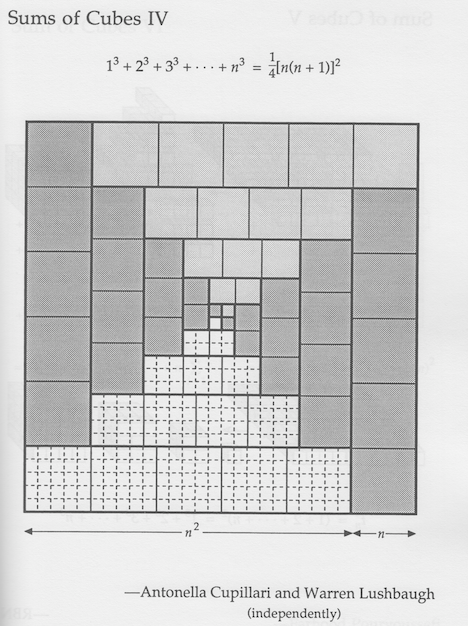
\includegraphics [scale=0.6] {sum_n3.png}\end{center}

\subsection*{Analysis}

We have shown in other write-ups, and you can easily verify by searching that the sum of the integers between $1$ and $n$ is 
\[ 1 + 2 + \dots + n = \sum\limits_{k=1}^n k = \frac{n(n+1)}{2} \]
The next one, the sum of the squares of the first $n$ integers, is useful for certain derivations in calculus (e.g. the Riemann sum to integrate $y=x^2$)
\[ 1^2 + 2^2 + \dots + n^2 = \sum\limits_{k=1}^n k^2 = \frac{n(n+1)(2n+1)}{6} \]
\[ = \frac{n^3}{3} + \frac{n^2}{2} + \frac{n}{3} \]
I was quite surprised to find that the sum of cubes is also simple and frankly, amazing
\[ 1^3 + 2^3 + \dots + n^3 = \sum\limits_{k=1}^n k^3 = \frac{n^2(n+1)^2}{2^2} = [\ \frac{n(n+1)}{2}\ ]^2 = [\ \sum\limits_{k=1}^n k \ ] ^2 \]
\begin{equation}
\boxed{ \sum\limits_{k=1}^n k^3 = [\ \sum\limits_{k=1}^n k \ ] ^2}
\end{equation}
Let's just try to prove the last formula using induction.

The "base case" is pretty simple.  For $n=2$
\[ 1^3 + 2^3 = 1 + 8 = 9 \]
and
\[ \frac{n^2(n+1)^2}{2^2} = \frac{2^2(3^2)}{2^2} = 3^2 = 9 \]
Check.  Now for the induction step what we need to show is that what we get assuming the formula for $n$ is correct and then adding the term $(n+1)^3$
\begin{equation}
\boxed{ \frac{n^2(n+1)^2}{2^2} + (n+1)^3}
\end{equation}
is equal to what we get by plugging $n+1$ into the formula.
\begin{equation}
\boxed{ \frac{(n+1)^2(n+2)^2}{2^2}}
\end{equation}
We need to show that eqn 2 is equal to eqn 3.  
\[ \frac{n^2(n+1)^2}{2^2} + (n+1)^3 = \frac{(n+1)^2(n+2)^2}{2^2} \]
First, we can factor out and cancel $(n+1)^2$ from both sides.  So then we have
\[ \frac{n^2}{2^2} + (n+1) \stackrel{?}{=} \frac{(n+2)^2}{2^2} \]
\[ n^2 + 4(n+1) \stackrel{?}{=} (n+2)^2 \]
Sure, that looks correct!  And we're done with the proof by induction, so we can put a little box.

$\square$

\subsection*{Looking deeper}
\[ \sum\limits_{k=1}^n k^3 = [\ \sum\limits_{k=1}^n k \ ] ^2 \]
I wanted to try to understand something more about why this is true.  A simple web search revealed the answer.  Here's an interesting pattern for the cubes of integers
\[ 1^3 = 1 \]
\[ 2^3 = 8 = 3 + 5 \]
\[ 3^3 = 27 = 7 + 9 + 11 \]
\[ 4^3 = 64 = 13 + 15 + 17 + 19 \]
\[ 5^3 = 125 = 21 + 23 + 25 + 27 + 29  \]

If you want a formula for $n^3$, notice that the first term is $n^2 - n + 1$ and the last term is $n^2 - n + 2n - 1$, and the number of terms for each sum equals $n$.  (There are $n$ odd numbers between $1$ and $2n-1$).

In other words, the sum of all the cubes of integers from $1^3$ to $n^3$ is equal to the sum of all the odd numbers up to $n^2 - n + 2n - 1 = n^2 + n - 1$.

How many of these numbers are there?  A little thought should convince you that the answer is $(n^2 + n)/2$.  For example, with $n=5$, our last odd number is $5^2 + 5 - 1 = 29$, and we have $(25 + 5)/2 = 15$ terms.

We want the sum of the first $(n^2 + n)/2$ odd numbers.

Let's look at another pattern
\[ 1 = 1 \]
\[ 2^2 = 4 = 1 + 3 \]
\[ 3^2 = 9 = 1 + 3 + 5 \]
\[ 4^2 = 16 = 1 + 3 + 5 + 7 \]
\[ 5^2 = 25 = 1 + 3 + 5 + 7 + 9 \]

The \emph{odd number theorem} says that the sum of the first $n$ odd numbers is equal to $n^2$.  We want the sum of the first $(n^2 + n)/2$ odd numbers, so that's $((n^2 + n)/2)^2$.  And that's how we get our formula.

\end{document}  